\documentclass{motivation}
  \usepackage{pst-pdf}
  \usepackage[ngerman,english]{babel}
  \usepackage[utf8x]{inputenc}
  \usepackage[T1]{fontenc}
  \usepackage{graphicx}
  \usepackage{xcolor,colortbl}
  \usepackage{enumerate}
  \pdfpageattr {/Group << /S /Transparency /I true /CS /DeviceRGB>>}
  \PassOptionsToPackage{cmyk}{xcolor}

\begin{document}
\pdfpageattr {/Group << /S /Transparency /I true /CS /DeviceRGB>>}

\title{Distance maps of transportation networks\\ {\ttlit web-based, interactive rendering and stylization}}

\subtitle{Conception and prototyping of an interactive rendering technique for distance maps based on OpenStreetMap graph data utilizing glTF tiles and WebGL.}

\numberofauthors{1}

\author{
  \alignauthor
  Alexander Schoedon, B.Sc\\
         \affaddr{Geoinformation and Visualization, M.Sc}\\
         \affaddr{Institute of Geography, Potsdam University}\\
         \email{schoedon@uni-potsdam.de}
}

\date{8 October 2015}

\maketitle
\pdfpageattr {/Group << /S /Transparency /I true /CS /DeviceRGB>>}

\begin{abstract}
  Different approaches for styling and rendering maps in web applications exist. Widely used architectures are raster or vector services that provide web mapping apps with geodata in client/server models. Raster data is efficiently prerendered server-side using a static, predefined layout. Vector data can be rendered client-side using dynamic layouts with CPU-consuming JavaScript postprocessing algorithms.\par
  In the light of powerful, dedicated graphics hardware being even available on mobile devices nowadays, this paper suggests new techniques for client-side rendering of web maps with complex geometries on GPUs. This technique allows to display complex geodata and maintain a dynamic, interactive layout while preserving real-time rendering performance and low response times.\par
  A proof-of-concept prototype implementation is attached to this paper to allow first insights in performance and feasibility.
\end{abstract}

\category{E.1.3}{Data}{Data Structures}[Graphs and networks]
\category{G.2.2}{Mathematics of Computing}{Discrete Mathematics}[Graph Theory]
\category{H.3.5}{Information Systems}{Information Storage and Retrieval}[Online Information Services]
\category{I.3.6}{Computing Methodologies}{Computer Graphics}[Methodology and Techniques]

\terms{Experimentation, Performance}

\keywords{Computergraphics, Geodata, Webmapping, Tiling, Distance Maps, Graph Network, WebGL, glTF}

\section{Introduction}

  \begin{figure}[h]
    \centering
    \includegraphics[width=0.475\textwidth]{resources/distmap.png}
    \caption{A possible distance map visualization.}
    \label{fig:distmap}
  \end{figure}

  Rendering transportation networks in web-based applications remains a performance critical task due to the complexity of the underlying geodata. An OpenStreetMap graph dataset snapshot of the Berlin/Brandenburg region as of October 2015 contains around 900,000 edges [22]. Using classic approaches to render such a huge dataset in a web browser either leaves users with a predefined, static layout (raster data) or a notable computation-intense rendering process (vector data).\par
  This paper proposes a new technology of web-based transportation network visualization with the application of line-based distance maps (compare figure \ref{fig:distmap}).

\subsection{Known issues}
  The two aforementioned solutions of styling and rendering web maps are widely established and have proven effective. But both approaches have certain drawbacks.\par
  Data transmitted in prerendered \textbf{raster} data formats (e.g. png, jpg) does not require any client-side processing and can be compressed and cached easily. This is used by major web mapping services like Google or Bing maps. The disadvantage for interactive mapping solutions is the lack of possibilities for users to dynamically interact with the map and retrieve custom layouts at runtime without requesting a full map tile reload. Web services using this technology solve this with tiny vector overlays displaying additional user-styled information. But it is not possible to interact with the map data itself.\par
  Geodata transmitted in \textbf{vector} formats (e.g. json, gml) opposes the raster tile approach and allows client-side stylization and rendering as the geographic raw data suddenly becomes available for the browser. But this advantage of options utilizing the geodata in the client comes with a major drawback in performance. Both the processing of the data and the rendering for the user are solved with CPU-consuming JavaScript algorithms\footnote{Some more recent solutions offer GPU-based rendering but fail with supplying convenient solutions of pre- or postprocessing of the vector data.}.

\subsection{Challenge}
  The challenge of this work is twofold interesting. On the one hand it is important to enable rendering using GPU-based techniques like WebGL [26]. This allows dynamic, interactive and user-defined layouts to be rendered directly on the client's device. But on the other hand it is a must to completely eliminate the client-side postprocessing of the geodata as this becomes a major performance bottleneck with increasing data complexity.\par
  The solution presented in this paper is a geometry-based approach rather than known vector- or raster-based solutions. It maintains the goal to allow real-time rendering with outstanding performance and very low response times for the client.

\section{Related work}
  A general motivation on web-based distance map applications in the context of geospatial analytics offers Hollburg et al. (2012) \cite{hollburghier}.\par
  Glander et al. (2010) researches on visualization of distance maps with focus on polygon-based approaches \cite{glandererreichbarkeitskarten}. Vaaraniemi et al. (2011) as well as Trapp et al. (2015) develop and evaluate solutions for transport network visualization utilizing modern computer graphics \cite{vaaraniemi2011high}\cite{trapp2014interactive}.\par
  Both Coughlin (2013) and Trevett (2013) deliver outstanding motivations on why we need a standardized data format close to hardware devices for 3D applications on the web \cite{coughlin3d}\cite{trevett20123d}.\par
  Altmaier et al. (2003) was among the first to outline issues in web-based geovisualization applications \cite{altmaier2003applications}. Klimke et al. (2011) proposed a camera path specification for geovisualization services on the web and mobile devices \cite{klimke2013service}.

\section{Implementation}
  The implementation is solved by an evolutionary prototyping process. The presented prototypes are therefore not compareable but rather help to outline issues with existing solutions and pave the way to the -- for this paper -- final solution utilizing glTF geometry tiles. Four prototypes are implemented:
  \begin{description}
    \item[Pt. \#1] Leaflet with native lines (JavaScript, GeoJSON)
    \item[Pt. \#2] Leaflet with canvas overlay (WebGL, GeoJSON)
    \item[Pt. \#3] Leaflet with viewport query (WebGL, GeoJSON)
    \item[Pt. \#4] Leaflet with geometry tiling (WebGL, glTF)
  \end{description}
  Prototype \#1 is not interesting for this work as it neither uses WebGL nor glTF and is only implemented to have a classic solution available. In addition, the performance of the first prototype is very poor, even for small distance maps (5 minutes travel time). It can be discarded directly.\par
  Prototype \#2 is interesting both for the successfull WebGL integration in Leaflet and the issues arising with GeoJSON postprocessing. See section \ref{sec:pt2} for more details.\par
  Prototype \#3 is utilizing viewport-based server requests on GeoJSON data. This approach is consuming too much bandwidth and server-capacities. Therefore, it is discarded in favour of a tile-based approach developed in the next step.\par
  Prototype \#4 is implementing a geometry tile service explicitly utilizing the glTF data exchange format. See section \ref{sec:pt4} for more details.

\subsection{Design decisions}
  Prior to implementation details, some design decisions on frameworks, data formats and geopraphic projections have to be discussed.

\subsubsection{Webmapping frameworks}
  This project focuses on the JavaScript webmapping framework \textit{Leaflet-JS} [15]. Better alternatives with a more advanced WebGL-integration are available (e.g. \textit{OpenLayers 3}) but a high compatibility with the existing \textit{Route360-JS} API developed by Motion Intelligence GmbH [24] is a requirement for this project. Therefore, Leaflet will be used.\par
  There is no native support for WebGL in Leaflet, yet\footnote{While writing this paper, a spanish software engineer, Iván Sánchez Ortega, started working on a Leaflet.GL plugin architecture [17] which was not taken into consideration as it is still experimental and was not available when this project implementation was started.}. Along with this implementation, a handful of Leaflet plugins will be developed which support a future WebGL integration [19][18] (see section \ref{sec:tile}).\par

\subsubsection{Data formats}
  Due to the data-intense applications in webmapping services, most implementations follow a client/server model. It's important to research and evaluate options on exchange formats for the underlying geodata.\par
  The following formats are considered worth for comparison.
  \begin{itemize}
  \item In computer graphics, the COLLADA digital asset exchange format (\texttt{.dae}) is used for modelling purposes and exchange of editable 3D models.
  \item The new OpenGL transfer fromat (\texttt{.gltf}) is currently being drafted by the Khronos Group [13] and promises to be a file format more close to the hardware requirements.
  \item In geoinformation sciences, GeoJSON is a JavaScript object notation (\texttt{.json}) which is extended by geographic features with geometries and properties.
  \item The Geography Markup Language (\texttt{.gml}) is an XML grammar for expressing geographical features.
  \end{itemize}
  Formats not taken into account are KML, Google's equivalent to GML, and TopoJSON, another JSON format with merged geometry fields. In addition, raster data formats are ignored as they do not store any extractable geometry information.\par
  Table \ref{tab:dataform} compares the stated formats and evaluates both, their space-complexity and postprocessing requirements. The space-complexity is important to evaluate the required bandwidth for the application. The postprocessing is the aforementioned bottleneck in performance of transforming geographic data into close-to-hardware array buffers for the GPUs.\par

  \begin{table}[!h]
    \centering
    \begin{tabular}{l|c|l}
      Format & Space-Complexity & Client-Postprocessing\\ \hline
      \cellcolor{yellow!15}.dae.gz & \cellcolor{green!15}\texttt{++} & \cellcolor{red!15}required, decompress \\
      \cellcolor{green!15}.bgltf & \cellcolor{green!15}\texttt{+o} & \cellcolor{green!15}not required \\
      \cellcolor{yellow!15}.gltf.gz & \cellcolor{green!15}\texttt{+o} & \cellcolor{yellow!15}decompress only \\
      \cellcolor{yellow!15}.dae & \cellcolor{yellow!15}\texttt{oo} & \cellcolor{red!15}required \\
      \cellcolor{yellow!15}.gltf & \cellcolor{red!15}\texttt{o-} & \cellcolor{green!15}not required \\
      \cellcolor{red!15}.json & \cellcolor{red!15}\texttt{o-} & \cellcolor{red!15}required \\
      \cellcolor{red!15}.gml & \cellcolor{red!15}\texttt{---} & \cellcolor{red!15}required \\
    \end{tabular}
    \caption{Comparison of data formats}
    \label{tab:dataform}
  \end{table}
  Concerning the space requirements, both glTF and COLLADA perform above average. Base of the comparison are the Cesium Milk Truck and Cesium Man by Analytical Graphics Inc [9]. The binary version of glTF (\texttt{.bgltf}) is even smaller than a gzipped version (\texttt{.gltf.gz}). Classic geodata formats fail in terms of space-complexity since both, JSON and XML formats are quite bloated.\par
  Concerning the client-side postprocessing requirements, only the OpenGL transfer format allows to store array buffers which eleminates any javascript processing other than requesting and reading the data. This is an obvious knockout criteria for the other candidates and therefore glTF will be considered the best choice for this application. Details on the postprocessing issues will be discussed in section \ref{sec:issue}.

\subsubsection{Geographic projections}
  \label{sec:pix}
  To minimize the processing of data and allow easy GL-transformations, it's important to reduce reprojections and avoid spherical units (e.g. degree, lat/lon).\par
  Leaflet uses the \texttt{EPSG:4326} standard projection which is the world geodetic system 1984 (WGS84) and uses a latitude/longitude coordinate format. This means, all programming interfaces of Leaflet return values in degree.\par
  Internally, Leaflet uses \texttt{EPSG:3857}, the web mercator projection, a metric system going back to Gerard Mercator's flat world map in 1569 [25]. It uses northing and easting as a measure of distance in meters from the equator and the prime meridian. This is already an advantage over WGS84 as it does not require computing-intense spheric transformations in calculations. Unfortunately, Leaflet does not allow access to the internal metric system without automatically triggering one or more reprojections from/to WGS84 [23].\par

  \begin{figure}[h]
    \centering
    \includegraphics[width=0.3\textwidth]{resources/earth-256.pdf}
    \caption{The world in 256 square pixels.}
    \label{fig:earth256}
  \end{figure}

  To simplify the geographic coordinates, all geographic references will be projected on a single tile of size 256*256 pixel with it's origin in the north-west corner (see figure \ref{fig:earth256}). In this reference system, the Brandenburg Gate in Berlin would be at pixel coordinate \texttt{[137.51253, 83.9612]}. This allows enough precision, moves as close as we can get to hardware-coordinates and is still device-independent.

\subsection{Prototype \#2 with GeoJSON}
  \label{sec:pt2}
  The 2nd Prototype is implementing Sumbera's Leaflet Canvas Overlay [14]. It is using a static local GeoJSON dataset with precalculated travel times for cars starting at the Brandenburg Gate in Berlin. The data is unfiltered but truncated at 15 minutes travel time (900 seconds) to limit file size and processing amount. The file is 8.8 MiB in size [10].

\subsubsection{Architecture}
  Leaflet provides a 2D \texttt{L.map()} canvas on a \texttt{<div id="map" />} HTML DOM element. This can be used for basic web mapping tools like raster base tiles or simple vector items. The extended class \texttt{L.canvasOverlay()} provides Leaflet with a 3D overlay which handles redrawing of the canvas and therefore allows basic WebGL context integration (figure \ref{fig:overlay}).

  \begin{figure}[h]
    \centering
    \special{ps: 0.4 .setopacityalpha}
    \includegraphics[width=0.3\textwidth]{resources/canvasoverlay.pdf}
    \caption{3D overlay on 2D map canvas.}
    \label{fig:overlay}
  \end{figure}

  On each map interaction, a \texttt{drawGL()} call will be triggered by the overlay. This function reads the underlying GeoJSON and extracts all geographic features. For each feature in the featureset, the algorithm checks the travel time properties and decides whether the feature is visible (below selected threshold) or not.\par
  Each visible feature will be converted to typed array buffers for vertices and colours. Each coordinate of the geometry has to be mapped to pixel coordinates (section \ref{sec:pix}).

\subsubsection{Viewport math}
  To display geographic coordinates on a GPU-rendered map, two major steps have to be performed.\par
  First, the geographic projection has to be transformed into a pixel projection. Therefore, the coordinate origin has to be moved to the topleft corner by translating it along the x-axis and the negative y-axis for half an equator. The units will be scaled from 40.075.016 meters to 256 pixels.

  \begin{figure}[h]
    \centering
    \includegraphics[width=0.3\textwidth]{resources/viewport.pdf}
    \caption{Viewport coordinates overview.}
    \label{fig:viewport}
  \end{figure}

  Finally, this pixel projection has to be made visible in the current viewport of the client's device. The device coordinate origin will be translated to the topleft corner of the visible viewport. The model view will be scaled using the current zoom level scale factor and visible canvas size.  The topleft corner of the map can be retrieved from Leaflet and used as an offset for the model view to translate to the displayed geometries (figure \ref{fig:viewport}).

\subsubsection{Client issues}
  \label{sec:issue}
  This implementation shows two issues.\par
  A blocking performance issue is the conversion from geodata to array buffers. For the mentioned dataset of only 15 minutes travel time this results in an iteration over 29.864 geographic features. In addition, the coordinates have to be iterated as well, leaving this example with 129.034 spheric conversions for 64.517 coordinates.\par
  Another problem is the unability to access the internal \texttt{EPSG :3857} metric coordinates from Leaflet. All positions have to be transformed using compute-intense spherical (degree) rather than optimized metric conversions [23].

\subsection{Prototype \#4 with glTF}
  \label{sec:pt4}
  A solution which eleminates client-side data processing is required. The 4th prototype implements a new geometry-tiling approach [11].\par
  Map tiles are a common way to divide map data into portions of similar size. A tile at zoom level 0 shows the full world. Zoom level divides the world in 4 tiles, zoom level 2 in 16 tiles, and so on.

\subsubsection{Geometry tiling}
   Table \ref{tab:tilopts} highlights the advantages of geometry tiling. The layout stays dynamic and can be adjusted at runtime by custom user inputs similar to vector tiling approaches.\par
   The data processing is moved from client-side to server-side similar to raster tiling approaches. The result is high runtime preformance with low latencies and the resulting geometries can be cached client-side.\par
   The rendering happens on dedicated graphic devices and ensures outstanding performance even for complex geodata sets.

  \begin{table}[!h]
    \centering
    \begin{tabular}{l|l|l|l}
      Tile & Layout & Processing & Rendering\\ \hline
      \cellcolor{yellow!15}Raster & \cellcolor{red!15}static & \cellcolor{green!15}Server & \cellcolor{red!15}Server\\
      \cellcolor{yellow!15}Vector & \cellcolor{green!15}dynamic & \cellcolor{red!15}Client/CPU & \cellcolor{green!15}Client/GPU\\
      \cellcolor{green!15}Geometry & \cellcolor{green!15}dynamic & \cellcolor{green!15}Server & \cellcolor{green!15}Client/GPU\\
    \end{tabular}
    \caption{Tiling options}
    \label{tab:tilopts}
  \end{table}
  Figure \ref{fig:geotile} shows a screenshot of a modified version of the 4th prototype. It displays the geometry tile \texttt{[2200,1343]} at zoom level 12 rendered with WebGL using random colours.

  \begin{figure}[h]
    \centering
    \includegraphics[width=0.475\textwidth]{resources/geometry-tile.png}
    \caption{Geometry tile rendered with WebGL.}
    \label{fig:geotile}
  \end{figure}

\subsubsection{Architecture}
  The current implementation requires a client/server architecture which offers both, a tiling service supplying the precalculated geometry tiles and a routing service supplying travel times on-request at runtime (figure \ref{fig:arch}).

  \begin{figure}[h]
    \centering
    \includegraphics[width=0.475\textwidth]{resources/arch.pdf}
    \caption{Architecture: tiling, routing, rendering.}
    \label{fig:arch}
  \end{figure}

  The tiling server regulary fetches OpenStreetMap snapshots and loads them into a PostGIS database. A tiling algorithm developed by Silbersiepe (2015) filters the geodata based on attributes and zoom level and pregenerates tiles for at least 20 zoom levels [27].\par
  A routing server operated by Motion Intelligence GmbH provides travel times based on the selected transportation type (e.g. car, bike, public transport) and a starting location. This data can be requested multiple times without the need to update the underlying geometry tiles again.

\subsubsection{Tile data structure}
  \label{sec:tile}
  Two Leaflet plugins are being developed to manage the tiling data logic [18].\par
  \begin{itemize}
    \item \texttt{L.TileBuffer} is the actual class for all geometry tiles. Each instance has the properties of \texttt{x}, \texttt{y} and \texttt{zoom}. In addition it stores the three required typed array buffers to render the tile with WebGL: a \texttt{Float32Array} for vertices, a \texttt{Uint16Array} for indices and a \texttt{Float32Array} for colours. This information is enough to render the complete tile in a single draw call.
    \item \texttt{L.TileBufferCollection} is a class which implements the basic tile caching logic. It has a \texttt{zoom} and a \texttt{size} property. In addition, it holds a collection of \texttt{L.Tile\-Buffer} objects for the current zoom level. As soon as the client requests a redraw of the scene, the collection can be rendered based on zoom and position of the visible tiles.
  \end{itemize}
  On each load event of a tile, Leaflet will request the geometry (vertices and indices) from the tiling server and the travel times (colours) from the routing server. These three arrays are recieved in glTF format. They are used to create \texttt{L.TileBuffer} objects (figure \ref{fig:tbuff}).

  \begin{figure}[h]
    \centering
    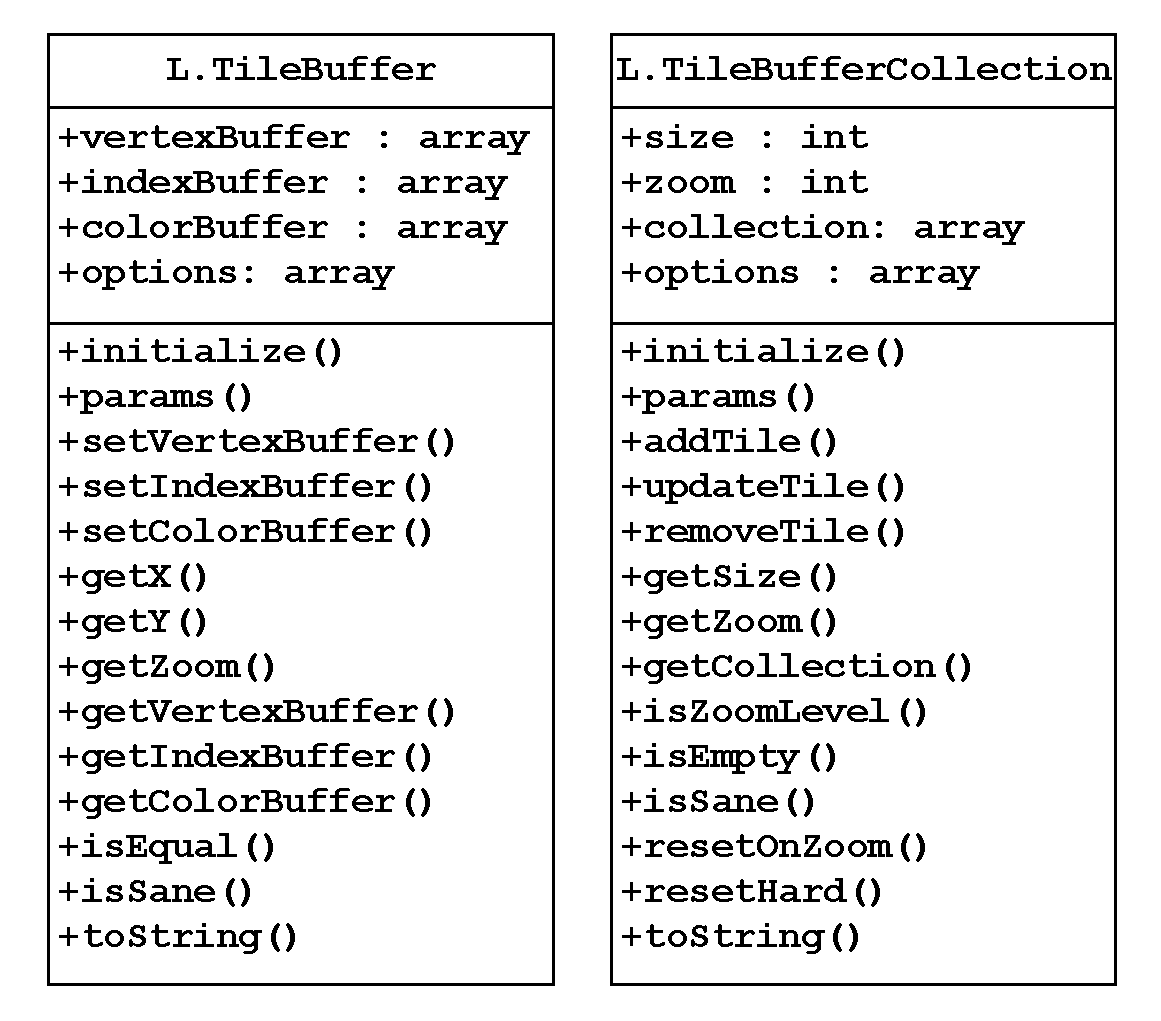
\includegraphics[width=0.3\textwidth]{resources/classes.pdf}
    \caption{Two Leaflet plugins for geometry tiling.}
    \label{fig:tbuff}
  \end{figure}

\subsubsection{Implementation status}
  This work focuses on frontend development only.\par
  The backend is operated by Motion Intelligence GmbH. The geodatabase with preprocessed OpenStreetMap graph data is available. The routing server API is available, too, but lacks of a working colour buffer (glTF) implementation for transportation networks. The tiling server is available but, unfortunately, is not serving glTF geometry tiles, yet.\par
  The frontend implementation is feature-complete. The Java\-Script tile cache and the WebGL rendering logic for geometry tiles is fully implemented with prototype \#4. The only piece missing is the glTF interface for the backend communication.

\section{Conclusions}
  A possible solution for a new approach of efficiently rendering and styling interactive web maps was demonstrated with the application focus on distance maps. Possible limitations were discovered and countermeasures developed.\par
  Geometry tiles utilizing preprocessed glTF data seem to be a promising way to render maps on both desktop and mobile devices. Future work should focus on developing a working glTF processing backend with tiling and routing server. On top of this, a fully working client/server infrastructure should be evaluated regarding it's performances. Results should be compared with classical raster or vector solutions.

\newpage
\appendix
\bibliographystyle{abbrv}
\bibliography{motivation}

\section{Related links}
  \begin{enumerate}[{[1]}]
  \setcounter{enumi}{8}
  \item Cesium Sample Models\\
    https://github.com/AnalyticalGraphicsInc/cesium/tree\\
    /c300529011714035cb254b493bf22b62ccf9da3d/Apps\\
    /SampleData/models
  \item Distance Maps Prototype \#2\\
    http://donschoe.github.io/leaflet-distance-maps-pt2/\\
    https://github.com/donSchoe/leaflet-distance-maps-pt2
  \item Distance Maps Prototype \#4\\
    http://donschoe.github.io/leaflet-distance-maps-pt4/\\
    https://github.com/donSchoe/leaflet-distance-maps-pt4
  \item GeoGL: The author's public blog\\
    http://geogl.ghost.io
  \item glTF draft specification\\
    https://github.com/KhronosGroup/glTF/blob/master
    /specification
  \item Leaflet canvas overlay\\
    http://bl.ocks.org/Sumbera/11114288\\
    https://github.com/donSchoe/L.CanvasOverlay
  \item Leaflet documentation\\
    http://leafletjs.com/reference.html
  \item Leaflet heatmaps\\
    https://github.com/Leaflet/Leaflet.heat
  \item Leaflet GL\\
    https://github.com/IvanSanchez/Leaflet.gl
  \item Leaflet tile buffer\\
    https://github.com/donSchoe/L.TileBuffer
  \item Leaflet WebGL\\
    https://github.com/donSchoe/Leaflet.WebGL
  \item Mapbox Raster Tiles\\
    https://www.mapbox.com/developers/api/maps/
  \item Mapzen Vector Tiles\\
    https://mapzen.com/projects/vector-tiles/
  \item OpenStreetMap\\
    https://www.openstreetmap.org
  \item Q: How to access Leaflet \texttt{EPSG:3857} coordinates?\\
    http://gis.stackexchange.com/q/153849/13692
  \item Route360 JS API\\
    https://developers.route360.net
  \item Time: Mercator World Map 1569\\
    http://ideas.time.com/2013/11/21/a-history-of-the-world-in-twelve-maps/slide/gerard-mercator-world-map-1569/
  \item WebGL specification\\
    https://khronos.org/registry/webgl/specs/latest
  \end{enumerate}

\section{Unpublished}
  \begin{enumerate}[{[1]}]
  \setcounter{enumi}{26}
  \item Silbersiepe, J. Web-based rendering of street networks. Spatial Analytics. Hasso-Plattner-Institute. 2015.
  \end{enumerate}

\section{Image credits}
  All tables in this paper are own work (tables \ref{tab:dataform}, \ref{tab:tilopts}). All figures are own graphics (figures \ref{fig:earth256}, \ref{fig:overlay}, \ref{fig:viewport}, \ref{fig:arch}, \ref{fig:tbuff}) or screenshots of own work (figures \ref{fig:distmap}, \ref{fig:geotile}).\par

  Background raster tiles are provided by Mapbox [20]. Vector data is provided by Motion Intelligence [24] and Mapzen [21].

\section{Acknowledgments}
  The author would like to thank Iván Sánchez Ortega, Stanis\-lav Sumbera and Vladimir Agafonkin for the inspiring pioneer work on Leaflet-WebGL integrations [17][14][16]. In addition, this work would not be possible without routing data provided by Henning Hollburg of Motion Intelligence GmbH (Route360 JS API) [24].

\section{Read more}
  Read more on the experiences with Leaflet and WebGL on the author's blog `GeoGL' [12].

\balancecolumns
\end{document}
